% ----------------------------------------
% LaTeX Article Template for CUED Reports by Jon Sowman, 2009 (jon@hexoc.com)
% ----------------------------------------

\documentclass[12pt]{article} % Set up the document class for an article
\usepackage[margin=2.5cm]{geometry}
%\usepackage{savetrees}		% Concise layout
\usepackage{amssymb}		% This packages permits using $ \therefore $
\usepackage{graphicx}		% SVG graphics includes, amongst other things
\usepackage{epstopdf}		% Allows EPS graphics includes
\usepackage{amsmath}		% This package allows the use of $ \text{} $
\usepackage{placeins}		% This package allows the use of \FloatBarrier
\usepackage{caption}		% This package allows subfigures:
\usepackage{subcaption}	    % And proper subfigure captioning
\usepackage{appendix}
\usepackage[amssymb]{SIunits}
\usepackage{xspace}
\usepackage{bold-extra}
\usepackage{tikz}

\usetikzlibrary{decorations.pathreplacing}
\usetikzlibrary{patterns}
\usetikzlibrary{calc}

\newcommand{\thegrid}{\textsc{the\textperiodcentered grid}\xspace}
\newcommand{\amaze}{\textsc{aMAZE}\xspace}

\title{\thegrid\\\small{\textsc{Large Interactive Display Field}}}
%\title {\textsc{emission}\\\large{\textsc{The Grid}}}
\author{\small{David Turner (dwt27@cl.cam.ac.uk)}\\
        \small{Adam Greig (ag611@eng.cam.ac.uk)}}
\date{} %Suppress date

% Begin the document
\begin{document}
\maketitle

\renewcommand{\abstractname}{Summary}
%%%%%%%%%%%%%%%%%%%%%%%%%%%%%%%%%%%%%%%%%%%%%%%%%%%%%%%%%%%%%%%%%%%%%%%%%%%
\begin{abstract}
Discover an immersive art/engineering installation comprising a forest of
radiant ``trees''.  As you move through \thegrid it senses your presence and
initiates a ripple of light and a susurration of subtle clicks, propogating
through the system.  Traverse your own maze of light or stand back and enjoy
the spectacle.

\vspace{5mm}

\thegrid is a $7\times7$ matrix of aluminium poles, illuminated by white LED
strips individually switched by a central controller.  User presence is
detected by an infrared computer vision system.  Applications include a
multiplayer virtual ``maze'', and interactive and passive display patterns.
\\
~
\\
\textbf{Requirements:} $14\metre \times 24\metre$ unlit ground, mains power
($1\kilo\watt$ peak).
\end{abstract}

\begin{figure}[h]
    \centering
    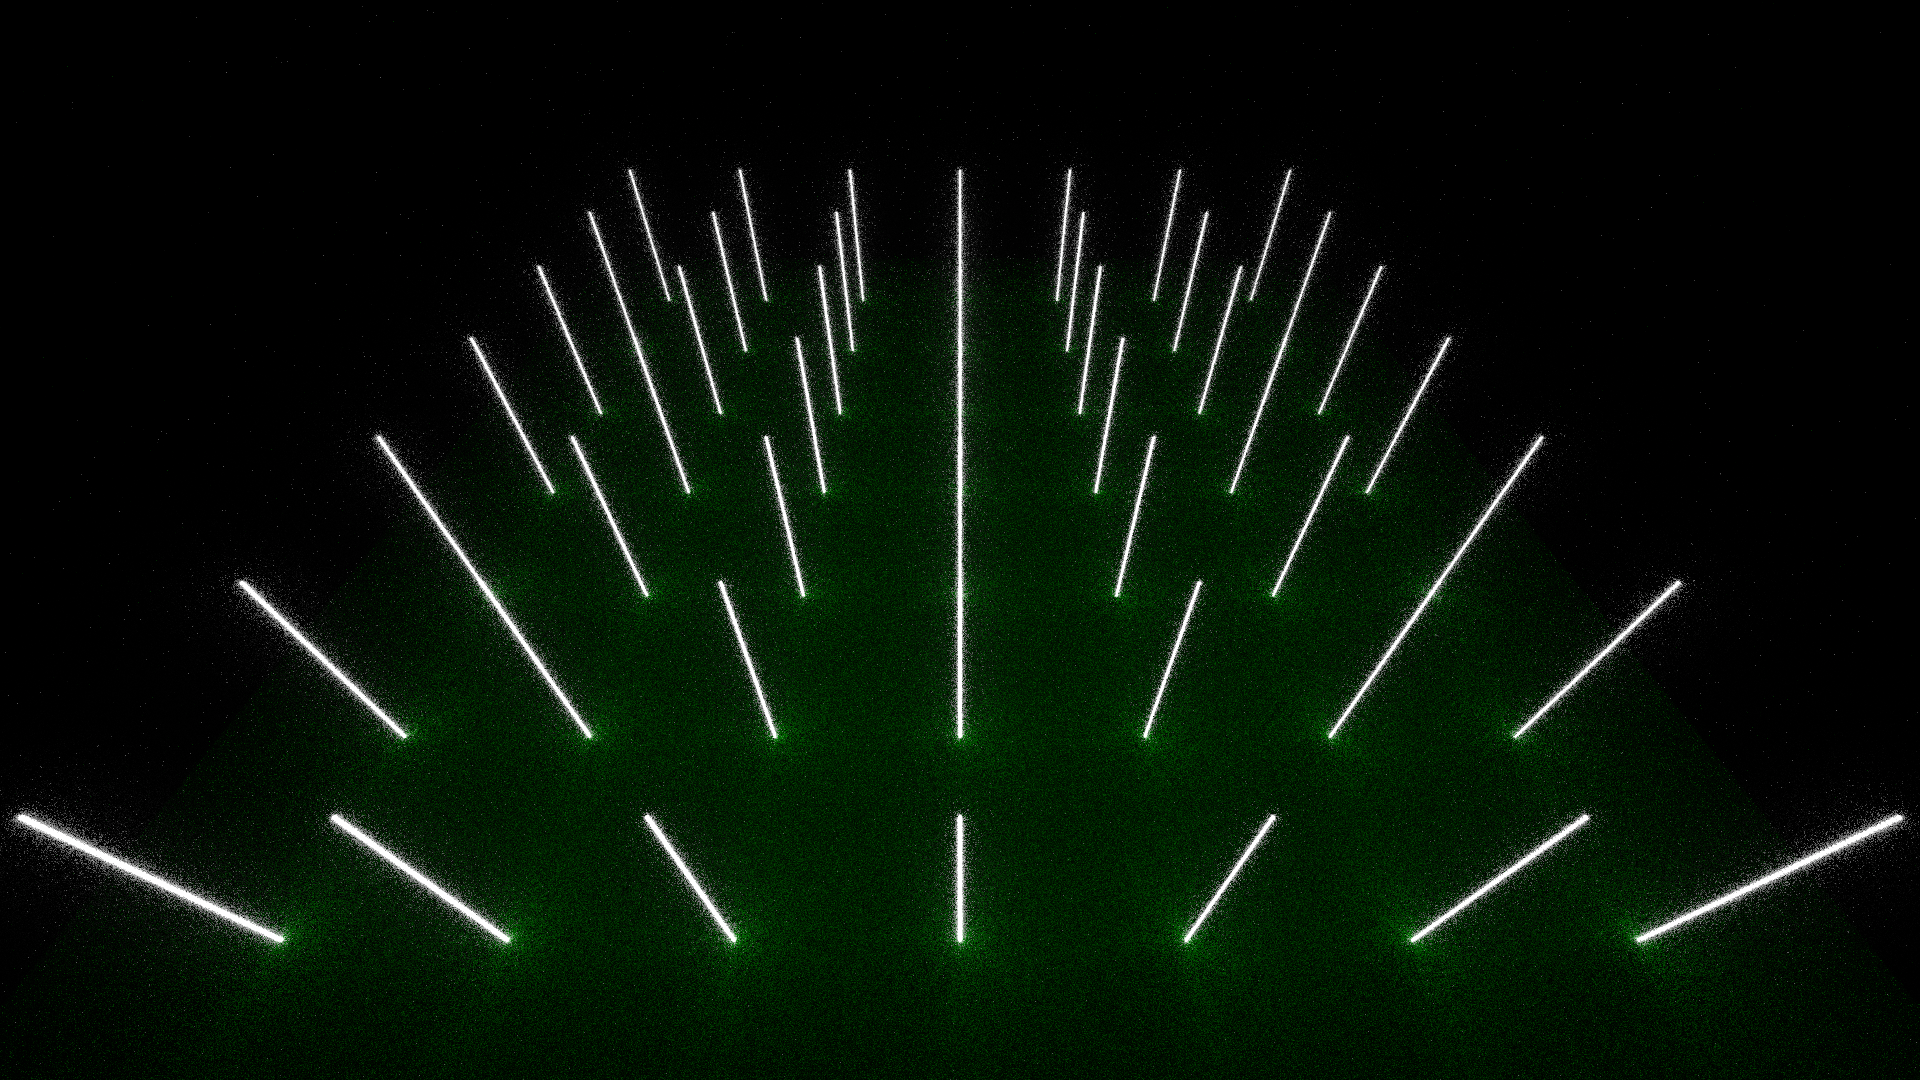
\includegraphics[width=\textwidth]{pics/render1.png}
    \caption{A computer graphics simulation of \thegrid.}
\end{figure}

%%%%%%%%%%%%%%%%%%%%%%%%%%%%%%%%%%%%%%%%%%%%%%%%%%%%%%%%%%%%%%%%%%%%%%%%%%%
\clearpage
\section{Design}
\subsection{Layout}
\thegrid occupies a space of approximately $24\metre \times 14\metre$.  Of
this, $12\metre \times 12\metre$ is the grid itself, consisting of a $7 \times
7$ grid of poles with $2\metre$ spacing.  A backstage area holds the power and
control tent as well as the camera mast.

\begin{figure}[h]
    \centering
    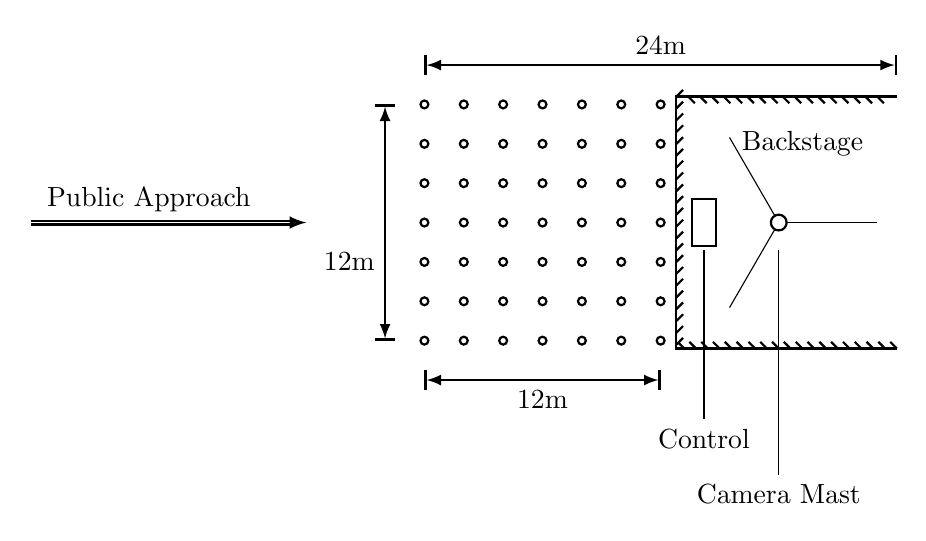
\begin{tikzpicture}[
        >=latex, thick,
    ]
    \foreach \x in {0.0cm, 0.5cm, 1.0cm, 1.5cm, 2.0cm, 2.5cm, 3.0cm}
        \foreach \y in {-1.5cm, -1.0cm, -0.5cm, 0.0cm, 0.5cm, 1.0cm, 1.5cm}
            \draw (\x, \y) circle (0.5mm) coordinate (\x\y);

    \draw (6.0cm, -1.6cm) -- (3.2cm, -1.6cm) -- (3.2cm, 1.6cm) -- (6.0cm, 1.6cm);
    \draw[decoration={border,segment length=1.5mm,amplitude=1.2mm,
                      mirror,angle=45},decorate]
         (6.0cm, -1.6cm) -- (3.2cm, -1.6cm) -- (3.2cm, 1.6cm) -- (6.0cm, 1.6cm);
    \draw (3.9cm, 1.0cm) node[right] {Backstage};

    \draw (3.4cm, -0.3cm) rectangle (3.7cm, 0.3cm) coordinate (control);
    \draw[thin] (3.55cm, -0.35cm) -- (3.55cm, -2.5cm) node[below] {Control};

    \draw[thin] (4.5cm, 0cm) -- ++(-0.625cm, -1.08cm);
    \draw[thin] (4.5cm, 0cm) -- ++(-0.625cm, 1.08cm);
    \draw[thin] (4.5cm, 0cm) -- ++(1.25cm, 0cm);

    \draw[fill=white] (4.5cm, 0.0cm) circle (1mm) coordinate (camera);
    \draw[thin] (4.5cm, -0.35cm) -- (4.5cm, -3.2cm) node[below] {Camera Mast};

    \draw[->, double] (-5.0cm, 0.0cm) -- (-1.5cm, 0.0cm);
    \draw (-3.5cm, 0.0cm) node[above] {Public Approach};

    \draw[|<->|] (0cm, -2.0cm) -- (3.0cm, -2.0cm);
    \draw (1.5cm, -2.0cm) node[below] {12m};

    \draw[|<->|] (-0.5cm, -1.5cm) -- (-0.5cm, 1.5cm);
    \draw (-0.5cm, -0.5cm) node[left] {12m};

    \draw[|<->|] (0cm, 2.0cm) -- (6.0cm, 2.0cm);
    \draw (3.0cm, 2.0cm) node[above] {24m};

    \end{tikzpicture}
    \caption{Plan schematic}
    \label{fig:planschematic}
\end{figure}

\subsection{Structural}
Each pole is $3\metre$ long, with $50\centi\metre$ being inserted into the
ground.  The poles are constructed from $\frac{3}{4}'' \times \frac{3}{4}''
\times \frac{1}{16}''$ aluminium angle section.  See
Appendix~\ref{app:engdrawings} for detailed drawings.

The interactivity camera will be mounted $8\metre$ above the ground on a pole,
guyed for rigidity.

\subsection{Electrical and Electronics}
\subsubsection{Cabling}
Each LED strip consumes $18\watt$ when active.  The wiring for one strip will
consist of twin core cable carrying power and return between the strip and the
control tent.  Additionally, a coaxial connection will run from the
interactivity camera to the control tent.

Ideally, all cabling inside \thegrid will be buried slightly below ground to
avoid a trip hazard.  If this is not possible, cabling could be run between the
tops of poles at a height of $2.5\metre$.

\subsubsection{Switching}
Each LED strip will be controlled using a MOSFET driver.  The drivers will be
switched by seven 8-output shift registers, themselves controlled by the CPU.

\subsubsection{Power}
The maximum power consumption of \thegrid will be $74\ampere$.  This will be
provided by four $550\watt$ ATX power supplies, each rated for $32\ampere$ on
its $+12\volt$ rail.

\subsection{Software and Control}
A laptop in the control tent will generate display patterns and handle
interactivity.  It will transmit lighting data via a serial link to an
microcontroller.  Upon receiving each frame, the microcontroller will clock the
data into the shift registers, then activate the output latch.

A night vision enabled camera mounted on a mast in the backstage area senses
movement and tracks the location of people inside \thegrid to co-ordiate
interactive applications and patterns.  Illumination will be provided by
several IR floodlights.

%%%%%%%%%%%%%%%%%%%%%%%%%%%%%%%%%%%%%%%%%%%%%%%%%%%%%%%%%%%%%%%%%%%%%%%%%%%
\section{Applications}
\subsection{\amaze}
\amaze is an interactive, virtual maze.  In this mode, when a user enters
\thegrid, a maze is randomly generated.  Squares the user can travel to are
lit, while squares representing walls are dark.  \amaze monitors the user's
progress and knows if the user completes the maze, or cheats!  The twist is
that \amaze only lights the user's square and adjacent squares---the user
cannot see ahead and can only explore passages by travelling them.

In multiplayer mode, two users can enter \thegrid simultaneously, each
navigating a different but overlapping maze, racing the other to victory.

\subsection{Interactive Patterns}
A number of interactive patterns will produce interesting visual effects based
on the movement of people in \thegrid, inspired by fluid disturbance and flow.

\subsection{Non-interactive Patterns}
For times when no users are directly interacting with \thegrid, non-interactive
patterns will display pre-programmed effects resembling waves, stars and
sparks.

%%%%%%%%%%%%%%%%%%%%%%%%%%%%%%%%%%%%%%%%%%%%%%%%%%%%%%%%%%%%%%%%%%%%%%%%%%%
\clearpage
\section{Risk Assessment}
\subsection{Mechanical}
\thegrid is an interactive exhibit and will involve people walking around a
structure in low lighting, however, there is a minimal risk of injury.  As
poles are embedded in soft ground and are constructed from thin aluminium
section, there is no serious risk of injury should somebody walk into a pole.

Poles will be $2.5\metre$ (8 foot 2 inches) tall, so there should be no risk of
impalement or eye injury.

In the very unlikely case of a pole falling on a person, the pole's light
weight (around $500\gram$) means there is minimal chance of injury.

With people walking around the installation in low light, there would be a
significant trip hazard were any cabling or guy-wires exposed.  For this
reason, all cabling inside \thegrid itself will be buried below the surface of
the ground.  If the cable cannot be buried, it will be run overhead between the
top of the poles.  Again, this is high enough that it will be impossible to
walk into.

The backstage area will contain cabling running at ground level alongside other
hazards and so will be off limits.

\subsection{Electrical}
All mains electronics will be contained within the control tent and power is
distributed through \thegrid at $12\volt$ DC\@.  The control tent will be
waterproof, and all exposed cabling, connections and electronics will be
waterproof.  The low voltage combined with RCD protection means there is a
minimal risk of electricution.

There is minimal risk of the low voltage LED strips in \thegrid itself posing a
fire hazard.  In the unlikely event of a fire in the control tent the hazard
would be contained in the off-limits backstage area, minimizing the risk to
users.

\subsection{Other}
In the event of a nearby thunder storm, the exposed metal poles could attract
lightning strikes (although the risk is  likely negligible compared to the main
NOC mast).  If there is a significant chance of a thunder storm, \thegrid will
be disconnected from the mains supply and placed off limits for the duration of
the storm.

There is a risk that individuals with photo-sensitive epilepsy could be
affected by \thegrid.  We will have to investigate further how to minimize this
risk, whether this be through appropriate warning signage or avoiding
problematic patterns such as flashing.

\clearpage
\section{Budget}

\begin{table}[ht]
    \centering
    \begin{tabular}{l|r|r|r}
        Item & Unit Cost (GBP) & Quantity & Subtotal (GBP) \\
        \hline
        $\frac{3}{4}''$ aluminium angle, 5m & 2.91 & 34 & 98.94\\
                 White LED strips, 5m & 1.83 & 50 & 91.45\\
$0.75\milli\metre^2$ cable, 100m reel, twin core & 17.88 & 6 & 107.28\\
                               Camera & 15.66 & 1 & 15.66\\
                               Camera Coax$^\dagger$ & 10.00 & 1 & 10.00\\
                              ATX PSU$^\dagger$ & 23.46 & 4 & 93.84\\
                       IR Floodlights & 27.99 & 2 & 55.98\\
                          Electronics$^\dagger$ & & & 50.00\\
                    Tent$^\ast$ & & & --\\
                   Camera mast \& guying$^\ast$ & & & --\\

                                &&&\\
                                &&&\\

                 \textbf{Total} & & & \textbf{523.15}\\

    \end{tabular}
\end{table}

$^\dagger$ Estimated price

$^\ast$ Already owned

\vspace{2cm}

While we are able to finance \thegrid personally, grants would be greatly
appreciated.

Some extension ideas that ended up being out of budget include addressable LED
strip and 5m tall poles.  We believe the current design obtains a good
compromise between cost and utility.

%%%%%%%%%%%%%%%%%%%%%%%%%%%%%%%%%%%%%%%%%%%%%%%%%%%%%%%%%%%%%%%%%%%%%%%%%%%
\clearpage
\begin{appendices}
\section{Engineering Drawings}
\label{app:engdrawings}

\begin{figure}[h]
    \centering
    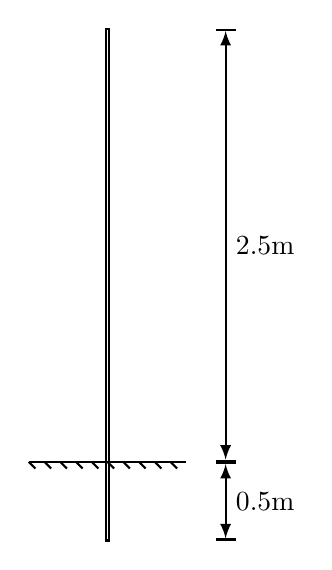
\begin{tikzpicture}[
        >=latex, thick,
    ]
    \draw (-1cm, 0cm) -- (1cm, 0cm);
    \draw[decoration={border,segment length=2mm,amplitude=1.2mm,
                      mirror,angle=45},decorate] (-1cm, 0cm) -- (1cm, 0cm);

    \draw (-0.19mm, -1cm) rectangle (0.19mm, 5.5cm);

    \draw[|<->|] (1.5cm, 0cm) -- (1.5cm, 5.5cm);
    \draw (1.5cm, 2.75cm) node[right] {$2.5\metre$};

    \draw[|<->|] (1.5cm, 0cm) -- (1.5cm, -1cm);
    \draw (1.5cm, -0.5cm) node[right] {$0.5\metre$};

    \end{tikzpicture}
    \caption{Side view of a single pole}
\end{figure}

\begin{figure}[h]
    \centering
    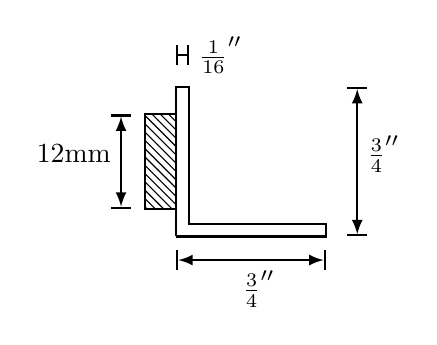
\begin{tikzpicture}[
        >=latex, thick,
    ]
    \draw (0mm, 0mm) -- (0mm, 19mm) -- (1.6mm, 19mm) --
          (1.6mm, 1.6mm) -- (19mm, 1.6mm) --  (19mm, 0mm) -- (0mm, 0mm);

    \draw[pattern=north west lines]
        (0mm, 3.5mm) -- (-4mm, 3.5mm) -- (-4mm, 15.5mm) -- (0mm, 15.5mm);

    \draw[|<->|] (0mm, -3mm) -- (19mm, -3mm);
    \draw (10.5mm, -3mm) node[below]{$\frac{3}{4}''$};

    \draw[|<->|] (23mm, 0mm) -- (23mm, 19mm);
    \draw (23mm, 10.5mm) node[right]{$\frac{3}{4}''$};

    \draw[|-|] (0mm, 23mm) -- (1.6mm, 23mm);
    \draw (1.6mm, 23mm) node[right]{$\frac{1}{16}''$};

    \draw[|<->|] (-7mm, 3.5mm) -- (-7mm, 15.5mm);
    \draw (-7mm, 10.5mm) node[left]{$12\milli\metre$};
    \end{tikzpicture}
    \caption{Top view of a single pole with LED strip}
\end{figure}


\begin{figure}[h]
      \centering
      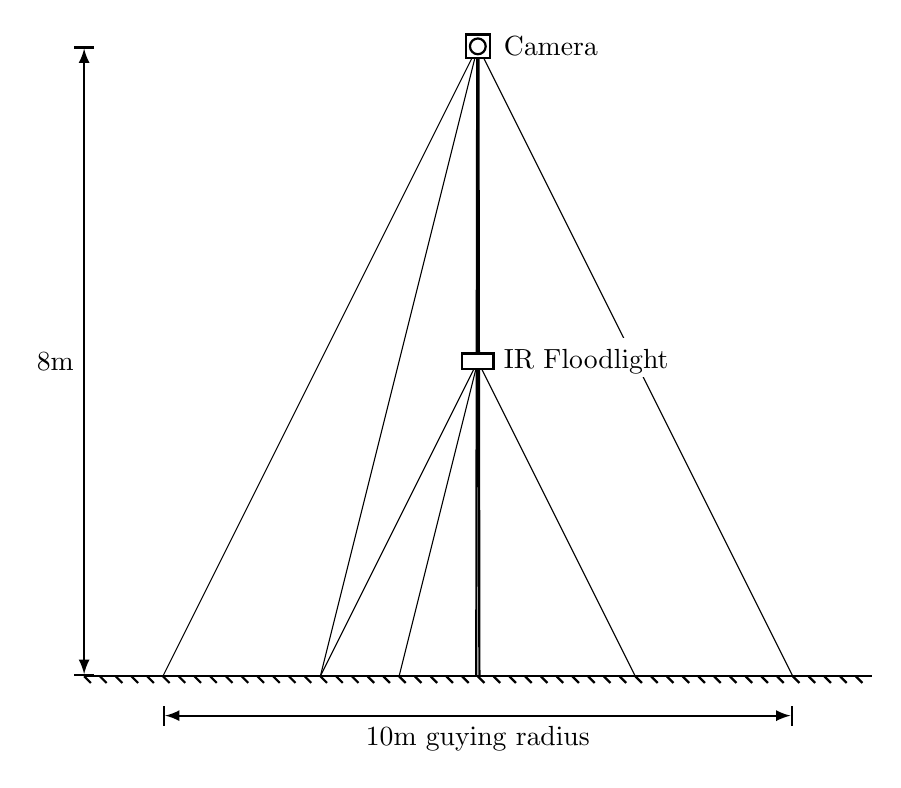
\begin{tikzpicture}[
          >=latex, thick,
      ]
      \draw (-5cm, 0cm) -- (5cm, 0cm);
      \draw[decoration={border,segment length=2mm,amplitude=1.2mm,
                        mirror,angle=45},decorate] (-5cm, 0cm) -- (5cm, 0cm);

      \draw (-0.2mm, 0) -- (-0.075mm, 8cm) -- (0.075mm, 8cm) -- (0.2mm, 0);

      \draw[thin] (0, 4cm) -- (-2cm, 0);
      \draw[thin] (0, 4cm) -- (-1cm, 0);
      \draw[thin] (0, 4cm) -- (2cm, 0);

      \draw[thin] (0, 8cm) -- (-4cm, 0);
      \draw[thin] (0, 8cm) -- (-2cm, 0);
      \draw[thin] (0, 8cm) -- (4cm, 0);

      \draw[|<->|] (-5cm, 0) -- (-5cm, 8cm);
      \draw (-5cm, 4cm) node[left] {8\metre};

      \draw[fill=white] (-0.2cm, 3.9cm) rectangle (0.2cm, 4.1cm);
      \draw[fill=white,draw=none] (1.8cm, 3.8cm) rectangle (2.3cm, 4.3cm);
      \draw (0.2cm, 4cm) node[right] {IR Floodlight};

      \draw[fill=white] (-0.15cm, 7.85cm) rectangle (0.15cm, 8.15cm);
      \draw[fill=white] (0, 8cm) circle (0.1cm);
      \draw (0.2cm, 8cm) node[right] {Camera};

      \draw[|<->|] (-4cm, -0.5cm) -- (4cm, -0.5cm);
      \draw (0cm, -0.5cm) node [below] {$10\metre$ guying radius};

      \end{tikzpicture}
      \caption{Side view of camera mast}
  \end{figure}

%%%%%%%%%%%%%%%%%%%%%%%%%%%%%%%%%%%%%%%%%%%%%%%%%%%%%%%%%%%%%%%%%%%%%%%%%%%
\clearpage
\section{Structural Design Verification}
The structural design can be verified quantitatively using Euler-Bernoulli beam
theory.  This assumes any deflection is small and that shear forces cause
negligible deflection.  These assumptions are justified when the beam concerned
is slender, i.e. its length is greater than 20 times its thickness, a condition
more than satisfied for \thegrid's poles.

From a basic structural point of view, \thegrid's poles are slender vertical
cantilevers subject to self weight and lateral wind loading.

\subsection{Basic Properties}
The following calculations are based on the beam's \emph{Second Moment of Area
in the U axis} ($I_{uu}$), \emph{Density} ($\rho$), and \emph{Young's Modulus}
($E$).  The U axis ($45^\circ$ from the X and Y axes) has the weakest second
moment of area (see Figure \ref{fig:iangle}).  The second moment of area in the
U axis is defined:

$$ I_{uu} = \int \! v^2 \, \mathrm{d}A $$

where the V axis is perpendicular to the U axis.  For thin walled equal angle
section:

$$ \mathrm{d}A = 2 t \sqrt{2} \, \mathrm{d}v $$
\begin{align*}
I_{uu} &= 2 t \sqrt{2} \int_{\frac{-a}{2\sqrt{2}}}^{\frac{a}{2\sqrt{2}}}
\! v^2 \, \mathrm{d}v \\
       &= \frac{2t\sqrt{2}}{3} \left[ y^3 \right]_{\frac{-a}{2\sqrt{2}}}
          ^{\frac{a}{2\sqrt{2}}} \\
       &= \frac{2t\sqrt{2}}{3} \left( \frac{a^3}{16\sqrt{2}} -
          \frac{-a^3}{16\sqrt{2}} \right) \\
       &= \frac{2t\sqrt{2}}{3} \left( \frac{a^3}{8\sqrt{2}} \right) \\
       &= \frac{ta^3}{12}
\end{align*}

\begin{figure}[h]
    \centering
    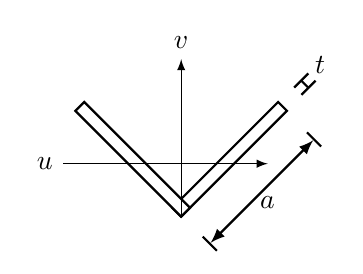
\begin{tikzpicture}[
            >=latex, thick,
    ]
    \draw[rotate=-45,fill=white] (0, 0) rectangle (-1.588mm, 19mm);
    \draw[rotate=45,fill=white] (0, 0) rectangle (1.588mm, 19mm);

    \draw[rotate=45, |<->|] (0, -5mm) -- (19mm, -5mm);
    \draw[rotate=45] (10.5mm, -5mm) node[below] {$a$};

    \draw[rotate=45, |-|] (23mm, 0mm) -- (23mm, 1.588mm);
    \draw[rotate=45] (23mm, 0.8mm) node[above right] {$t$};

    \draw[thin,->] (-15mm, 6.72mm) -- (11mm, 6.72mm);
    \draw (-15mm, 6.72mm) node[left] {$u$};

    \draw[thin,->] (0mm, 0mm) -- (0mm, 20mm);
    \draw (0mm, 20mm) node[above] {$v$};
    \end{tikzpicture}
    \caption{Second Moment of Area for Angle Section}
    \label{fig:iangle}
\end{figure}

For $a=\frac{3}{4}''$ and $t=\frac{1}{16}''$,
$I = 9.15\times10^{-10}~\metre^4$.

Standard values for the density and Young's Modulus of aluminium are used,
$\rho=2,700\kilo\gram/\metre$, $E = 69 \times 10^9 \giga\pascal$.

\subsection{Flexural Rigidity}
A simple test of a beam's rigidity is its deflection under self weight when
mounted as a horizontal cantilever.  For a horizontal cantilever of length $L$
with distributed loading $w$, the deflection is:

\begin{equation}
\delta = \frac{w L^4}{8EI}
\label{eq:cantilever}
\end{equation}

\begin{figure}[h]
    \centering
    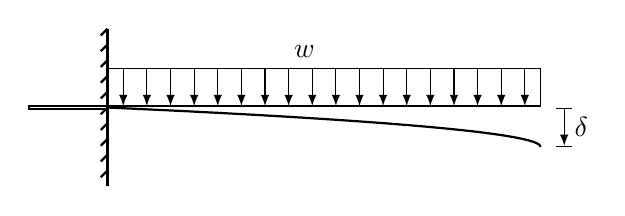
\begin{tikzpicture}[
        rotate=-90, >=latex, thick,
    ]
    \draw (-1cm, 0cm) -- (1cm, 0cm);
    \draw[decoration={border,segment length=2mm,amplitude=1.2mm,
                      mirror,angle=45},decorate] (-1cm, 0cm) -- (1cm, 0cm);

    \draw (-0.19mm, -1cm) rectangle (0.19mm, 0cm);
    \draw (5mm, 5.5cm) parabola (0mm, 0cm);

    \draw (-0.5cm, 2.5cm) node[above]{$w$};

    \draw[thin] (-0.5cm, 0) rectangle (-0.19mm, 5.5cm);

    \foreach \y in {0.2, 0.5, ..., 5.5}
        \draw[thin,->] (-0.5cm, \y) -- (-0.19mm, \y);

    \draw[thin,|->|] (0cm, 5.8cm) -- (0.5cm, 5.8cm);
    \draw (0.25cm, 5.8cm) node[right] {$\delta$};

    \end{tikzpicture}
    \caption{Horizontal cantilever deflection due to self weight}
\end{figure}

Applying a loading of $1.60~\newton/\metre$ for the weight of aluminium and
$0.374~\newton/\metre$ for the LEDs, we get a total loading of
$w=1.97~\newton/\metre$ and a deflection of $\delta = 0.153~\metre$.

\subsection{Buckling}
Slender columns under a compressive load will tend to fail by buckling rather
than crushing.  The standard formula for the maximum load (applied at the tip
of the column) due to Euler buckling is:

$$ F_{\text{crit}} = \frac{\pi^2 EI}{(KL)^2} $$

\begin{figure}[h]
    \centering
    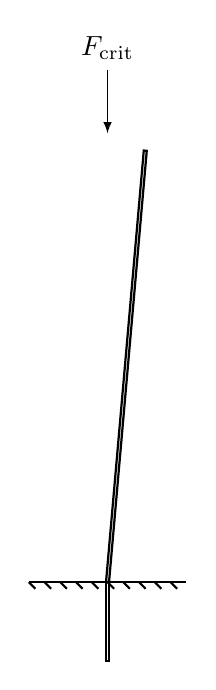
\begin{tikzpicture}[
        >=latex, thick,
    ]
    \draw (-1cm, 0cm) -- (1cm, 0cm);
    \draw[decoration={border,segment length=2mm,amplitude=1.2mm,
                      mirror,angle=45},decorate] (-1cm, 0cm) -- (1cm, 0cm);

    \draw (-0.19mm, -1cm) rectangle (0.19mm, 0cm);
    \draw[rotate around={-5:(0,0)}] (-0.19mm, 0cm) rectangle (0.19mm, 5.5cm);

    \draw[thin,->] (0, 6.5cm) -- (0, 5.7cm);
    \draw (0, 6.5cm) node[above] {$F_{\text{crit}}$};

    \end{tikzpicture}
    \caption{Euler buckling of pole}
\end{figure}

$(KL)$ is the effective length, determined by boundary conditions.  \thegrid's
poles are vertical cantilevers, for which the correction factor is $K=2$.  For
these poles, the critical force due to buckling is $F_{\text{crit}} =
24.9~\newton$, or $2.54~\kilo\gram$.

The total weight of the aluminium and LEDs is far less than $2.54~\kilo\gram$
and the self-weight loading is distributed rather than applied at the tip, so
there is no risk of buckling under self weight.

\subsection{Wind Loading}
Wind loading upon the poles can be modelled as a vertical cantilever subject to
lateral uniform distributed loading.  The loading depends on the wind speed and
lateral cross sectional area of the pole.  At $13.4~\metre/\second$ ($30$~mph),
loading is $119~\newton/\metre^2$, and at $17.9~\metre/\second$ ($40$~mph),
loading is $268~\newton/\metre^2$.  The maximum lateral cross sectional area of
the pole is $0.0674~\metre^2$.

Using Equation \ref{eq:cantilever}, we find that $30$~mph and $40$~mph winds
give deflection of $0.248~\metre$ and $0.559~\metre$ respectively.

\begin{figure}[h]
    \centering
    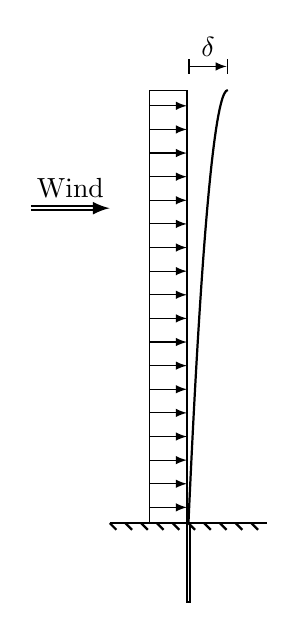
\begin{tikzpicture}[
        >=latex, thick,
    ]
    \draw (-1cm, 0cm) -- (1cm, 0cm);
    \draw[decoration={border,segment length=2mm,amplitude=1.2mm,
                      mirror,angle=45},decorate] (-1cm, 0cm) -- (1cm, 0cm);

    \draw (-0.19mm, -1cm) rectangle (0.19mm, 0cm);
    \draw[thick] (5mm, 5.5cm) parabola (0mm, 0cm);

    \draw[->,double] (-2cm, 4.0cm) -- (-1cm, 4.0cm);
    \draw (-1.5cm, 4.0cm) node[above]{Wind};

    \draw[thin] (-0.5cm, 0) rectangle (-0.19mm, 5.5cm);

    \foreach \y in {0.2, 0.5, ..., 5.5}
        \draw[thin,->] (-0.5cm, \y) -- (-0.19mm, \y);

    \draw[thin,|->|] (0cm, 5.8cm) -- (0.5cm, 5.8cm);
    \draw (0.25cm, 5.8cm) node[above] {$\delta$};

    \end{tikzpicture}
    \caption{Wind loading on pole}
\end{figure}



\FloatBarrier
\clearpage
\section{Cable layout}
\begin{figure}[h]
    \centering
    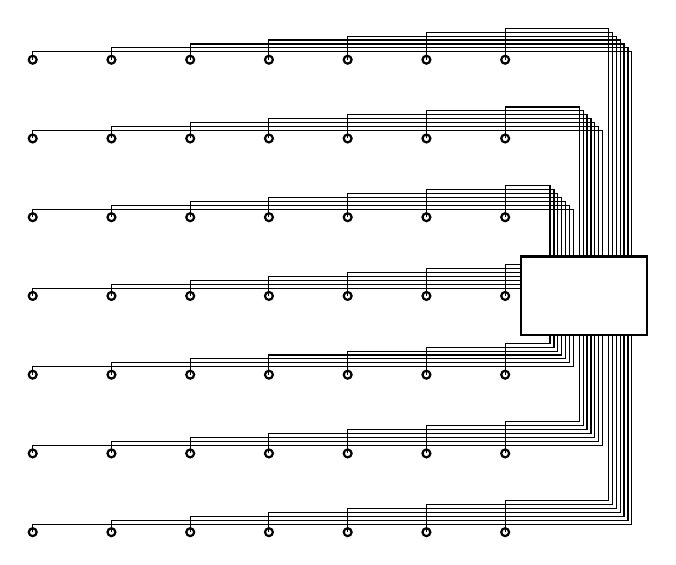
\begin{tikzpicture}[
        >=latex, thick,
    ]

    \foreach \x in {0cm, 1cm, 2cm, 3cm, 4cm, 5cm, 6cm}
        \foreach \y in {-3cm, -2cm, -1cm, 0cm, 1cm, 2cm, 3cm}
            \draw (\x, \y) circle (0.5mm);

    \foreach \x in {0cm, 1cm, 2cm, 3cm, 4cm, 5cm, 6cm}
        \foreach \y in {-3cm, -2cm, -1cm, 0cm, 1cm, 2cm, 3cm}
            \draw[thin] (\x, \y) -- (\x, \y + 1mm + \x/20) --
                  ($(6.5cm, \y) + (0, \x/20 + 1mm) - (\x/20, 0) + abs(\y)*(0.13mm, 0)$)
                  -- ++(0, -\y);

    \draw[fill=white] (6.2cm, -0.5cm) rectangle (7.8cm, 0.5cm);


    \end{tikzpicture}
    \caption{Power/control cable routing}
\end{figure}


\section{Electrical Design Verification}
\subsection{Power and Current Consumption}
The power consumption of the LED strip is $7.2~\watt/\metre$.  For 49 poles,
this gives a total peak power consumption of $882~\watt$.  Using Ohm's Law and
the definition of electrical power:

$$ V = IR $$
$$ P = VI $$

the maximum current flow in \thegrid is $73.5~\ampere$ at $12~\volt$ DC,
although no single conductor carries the entire current.

\subsection{Cabling Resistance and Voltage Drop}
Cabling between the control tent and poles will be 2-core cable with an area of
$0.75\milli\metre^2$, or $7.5 \times 10^{-7}~\metre^2$ per conductor.  The
resistivity of copper is $1.68 \times 10^{-8}~\ohm\metre$ at room temperature.
With a maximum cable length of around $20~\metre$ the total conductor length is
$40~\metre$, giving a resistance of $0.896~\ohm$.  With a current of
$1.5~\ampere$ per pole, this gives a voltage drop of $1.34~\volt$.

\clearpage
\section{Preliminary Testing}
A prototype pole was constructed from $20\milli\metre \times 20\milli\metre
\times 1.5\milli\metre$ aluminium section (c.f. $19\milli\metre \times
19\milli\metre \times 1.59\milli\metre$ for the final design).  We attached RGB
LED strip powered by a bench power supply.  This test confirmed the structural
rigidity of the pole design as well as the effectiveness of lighting with
30LED/$\metre$ strip.  We also confirmed the acceptable voltage range of the
LED strip.

\begin{figure}[h]
    \centering
    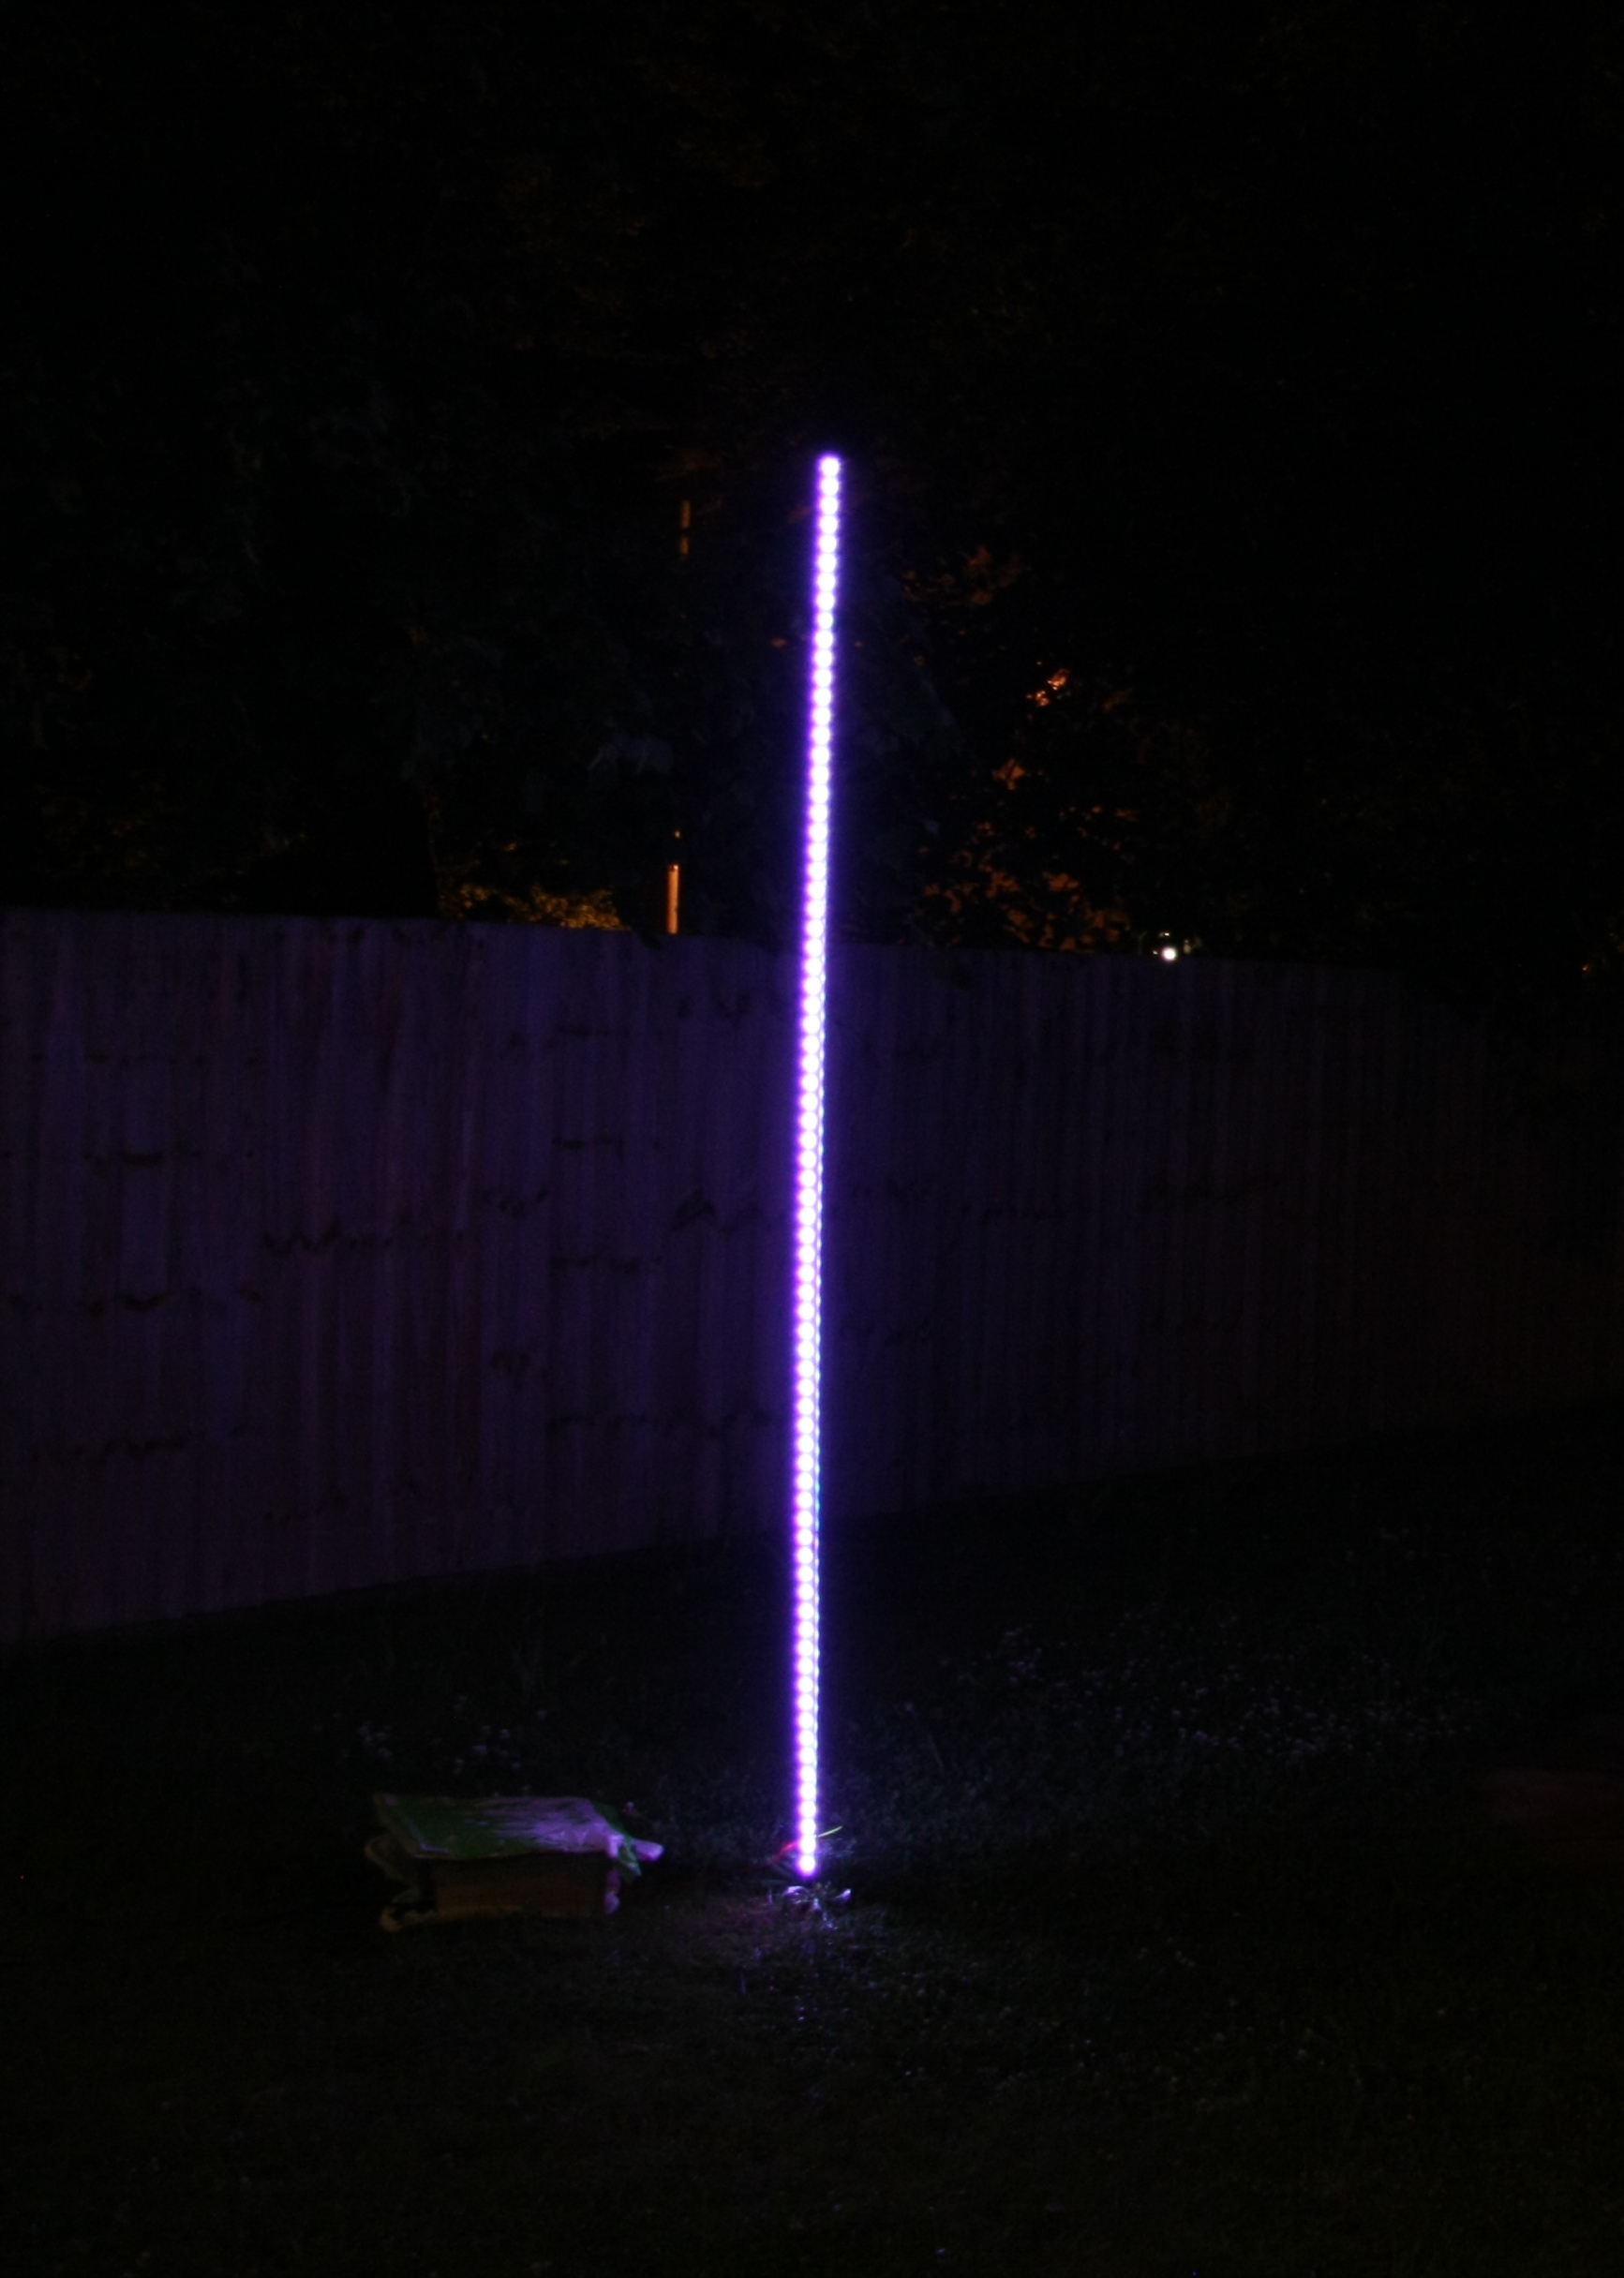
\includegraphics[height=15cm]{pics/protopole.jpg}
    \caption{Prototype pole}
\end{figure}

\clearpage
To verify the basis of the computer vision system, a night vision camera at a
height of $4\metre$ was used to observe a person at a distance of $10\metre$,
with and without an additional IR flood-light.

\begin{figure}[h]
    \centering
    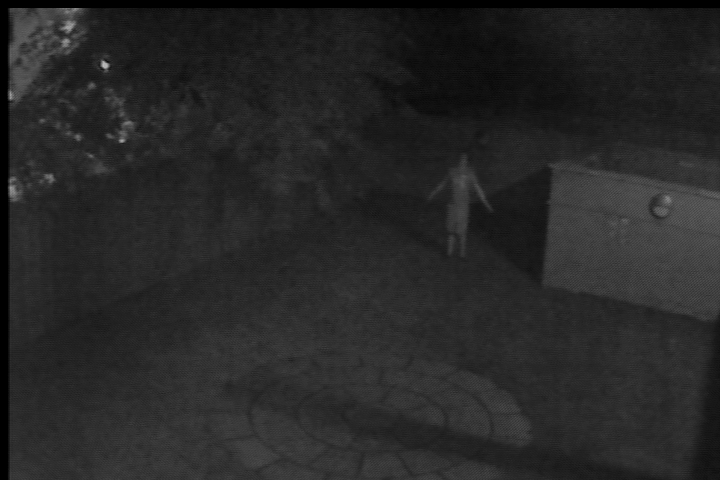
\includegraphics[width=10cm]{pics/ir_no_flood.png}
    \caption{Night vision camera without IR flood-light}
\end{figure}

\begin{figure}[h]
    \centering
    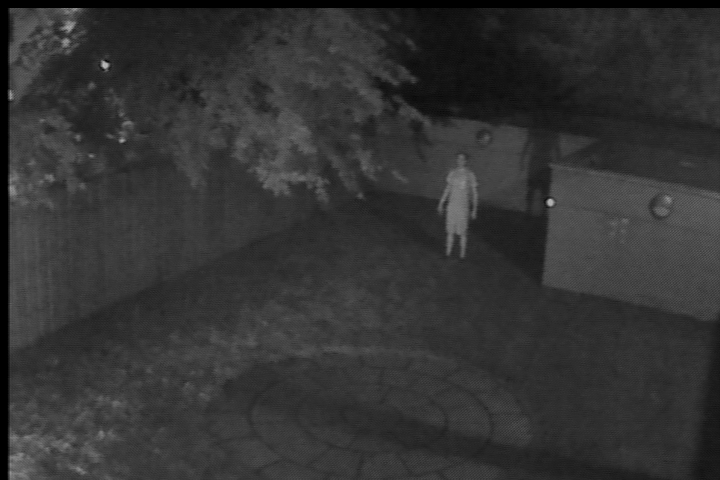
\includegraphics[width=10cm]{pics/ir_flood.png}
    \caption{Night vision camera with IR flood-light}
\end{figure}

$12\volt$ relays with $10\ampere$ rated contact current were found to give a
satisfying click.

\end{appendices}
\end{document}

